\section{Introduction}
%
In this project, we aim to establish a scope which covers two fields: \emph{robotics} and \emph{deep learning}.\\

In the last decades, robots have become a powerful allied to humans, as they are leveraged to perform all kind of tasks (hazardous explorations, personal assistance, cleaning, driving, \dots). However, we aim to design them to perform these tasks on the most autonomous way possible, which means not requiring to be controlled on every action (with exceptions, such as surgeon robots). This requires to provide robots a certain intelligence and capabilities to correctly trigger the most suitable action for each possible input stimulus. For this purpose, we can find multiple approaches for different problems (navigation, conversation, \dots).\\

Concretely, this article is dovetailed with \emph{Computer Vision}, which involves connecting cameras to a robot, and taking advantage of this on an autonomous way. Concretely, we will tackle the \emph{person following} challenge, which is based on a behavior governed by a person \emph{detection} system. Many approaches are already existing, such as color filters \cite{rocapal}, or disparities filtering. However, promising \emph{Deep Learning} techniques excel on their image processing variant, as they offer high quality results, accompanied by \emph{robustness} facing lighting issues (Fig. \ref{fig:intro_harsh_light}). This is the set of techniques we have used on this project, so we will describe the basis firstly.\\

\begin{figure}[h]
	\centering
	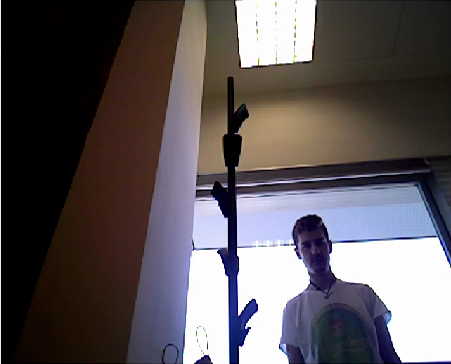
\includegraphics[width=2in]{images/light_ko_2}
	\caption{Harsh lighting situation for \emph{Computer Vision} algorithms.}
	\label{fig:intro_harsh_light}
\end{figure}


In the image detection quandary, the main objective is to determine \emph{presence and position} of a certain object in a given image. For this, we make use on this article of \emph{deep learning} techniques, concretely \emph{Convolutional Neural Networks} (CNNs).\\


This investigation has focused on exploring the synergies existing the two explained fields, making use of \emph{deep learning} to automatically command a robot to follow a determined person. This is achieved making use of two different modules: a \emph{perception} one, focused on the computer vision/deep learning tasks, and an \emph{actuation} module, which implements a case-based behavior, depending on what the perceptive part senses and computes. The designed system has been experimentally validated, as it will be seen on section \ref{sec:experiments}